% `template.tex', a bare-bones example employing the AIAA class.
%
% For a more advanced example that makes use of several third-party
% LaTeX packages, see `advanced_example.tex', but please read the
% Known Problems section of the users manual first.
%
% Typical processing for PostScript (PS) output:
%
%  latex template
%  latex template   (repeat as needed to resolve references)
%
%  xdvi template    (onscreen draft display)
%  dvips template   (postscript)
%  gv template.ps   (onscreen display)
%  lpr template.ps  (hardcopy)
%
% With the above, only Encapsulated PostScript (EPS) images can be used.
%
% Typical processing for Portable Document Format (PDF) output:
%
%  pdflatex template
%  pdflatex template      (repeat as needed to resolve references)
%
%  acroread template.pdf  (onscreen display)
%
% If you have EPS figures, you will need to use the epstopdf script
% to convert them to PDF because PDF is a limmited subset of EPS.
% pdflatex accepts a variety of other image formats such as JPG, TIF,
% PNG, and so forth -- check the documentation for your version.
%
% If you do *not* specify suffixes when using the graphicx package's
% \includegraphics command, latex and pdflatex will automatically select
% the appropriate figure format from those available.  This allows you
% to produce PS and PDF output from the same LaTeX source file.
%
% To generate a large format (e.g., 11"x17") PostScript copy for editing
% purposes, use
%
%  dvips -x 1467 -O -0.65in,0.85in -t tabloid template
%
% For further details and support, read the Users Manual, aiaa.pdf.


% Try to reduce the number of latex support calls from people who
% don't read the included documentation.
%


\typeout{}\typeout{If latex fails to find aiaa-tc, read the README file!}
%


\documentclass[]{aiaa-tc}% insert '[draft]' option to show overfull boxes
\usepackage{float}
\usepackage{epstopdf}
\usepackage{amsmath}
\usepackage[table,xcdraw]{xcolor}

\title{Zeus: Mission to Jupiter}

\author{
	Johnathan Clouse%
	\thanks{Graduate Student, Aerospace Engineering Sciences, 1111 Engineering Drive, Boulder, CO, 80309-0429}\\
	{\normalsize\itshape
		University of Colorado, Boulder, CO, 80309-0429, USA}
}

% Define commands to assure consistent treatment throughout document
\newcommand{\eqnref}[1]{(\ref{#1})}
\newcommand{\class}[1]{\texttt{#1}}
\newcommand{\package}[1]{\texttt{#1}}
\newcommand{\file}[1]{\texttt{#1}}
\newcommand{\BibTeX}{\textsc{Bib}\TeX}

\usepackage[euler]{textgreek}
\usepackage[colorlinks=true]{hyperref}
\hypersetup{urlcolor=cyan}

\usepackage{listings}
\usepackage{color} %red, green, blue, yellow, cyan, magenta, black, white
\definecolor{mygreen}{RGB}{28,172,0} % color values Red, Green, Blue
\definecolor{mylilas}{RGB}{170,55,241}

\usepackage{tablefootnote}
\usepackage{graphicx}
\usepackage{amsmath}
\usepackage{bm}
\usepackage{subfigure}
%\usepackage{subcaption}

\definecolor{mylilas}{RGB}{170,55,241}

% See p.105 of "TeX Unbound" for suggested values.
% See pp. 199-200 of Lamport's "LaTeX" book for details.
%   General parameters, for ALL pages:
\renewcommand{\topfraction}{0.9}	% max fraction of floats at top
\renewcommand{\bottomfraction}{0.8}	% max fraction of floats at bottom
%   Parameters for TEXT pages (not float pages):
\setcounter{topnumber}{2}
\setcounter{bottomnumber}{2}
\setcounter{totalnumber}{4}     % 2 may work better
\setcounter{dbltopnumber}{2}    % for 2-column pages
\renewcommand{\dbltopfraction}{0.9}	% fit big float above 2-col. text
\renewcommand{\textfraction}{0.07}	% allow minimal text w. figs
%   Parameters for FLOAT pages (not text pages):
\renewcommand{\floatpagefraction}{0.7}	% require fuller float pages
% N.B.: floatpagefraction MUST be less than topfraction !!
\renewcommand{\dblfloatpagefraction}{0.7}	% require
    \makeatletter
    \renewcommand\l@section{\@dottedtocline{2}{1.5em}{3em}}
    \makeatother
    
\begin{document}
	

	
	\maketitle
	
	\begin{abstract}
		\noindent 
		
	\end{abstract}
	
	\newpage
	
	\tableofcontents
	
	\newpage

	\section{Introduction}
Jupiter is the largest planet in the solar system, and the closest gas giant to the sun. 

A VEEJ (Venus-Earth-Earth-Jupiter) trajectory was considered for launch in 2020. The requirements are outlined as follows:
	
%	\begin{figure}[H]
%		\centering
%			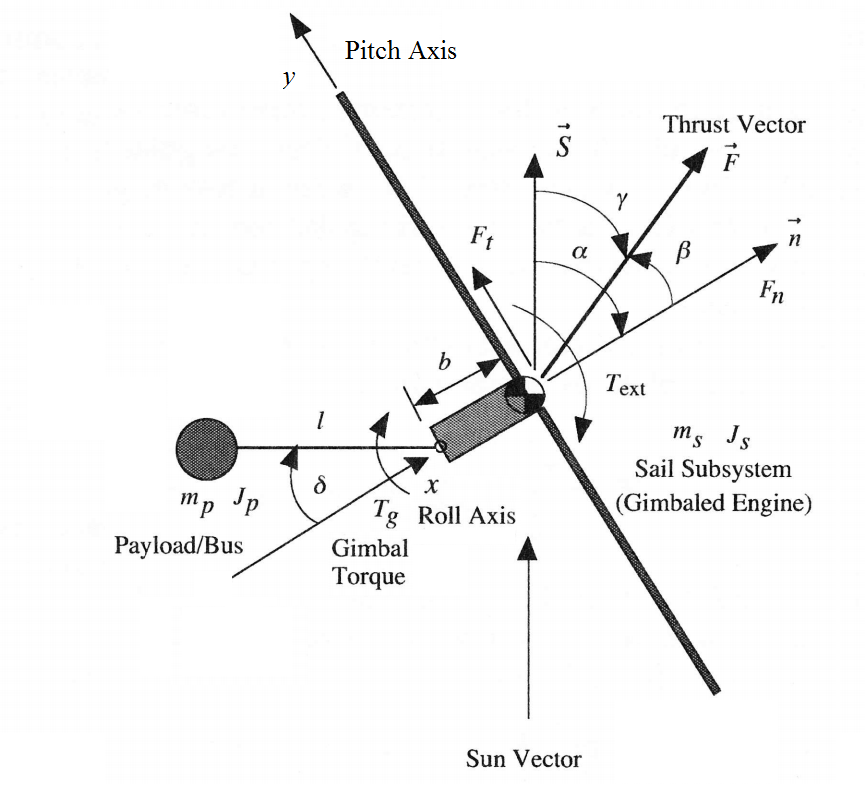
\includegraphics[width = 7.5cm]{schematic.png}
%		\caption{Diagram of the spacecraft\cite{WieSolarSail2}. }
%		\label{fig:Diagram}
%	\end{figure}	
	
	\vspace{5 mm}
	
The sailcraft's actuator was a gimbaled control boom between the sail subsystem and the spacecraft bus, which contained the majority of the spacecraft mass.  With the center of mass between the thrust point and the sun, expected disturbances would cause oscillation about some angle between the sun and the axis normal to the sail, $\alpha$, for a locked gimbal.  Changing the gimbal angle, $\delta$, would dampen this oscillation with the right control law. Roll and pitch angles were held to zero for this analysis. Sun sensors determined spacecraft yaw, and had a maximum error of $\pm$0.05$^{\circ}$.
	
	\vspace{5 mm}

The state-space model had four states: the sun angle ($\alpha$), the rate of the sun angle ($\dot{\alpha}$), the gimbal angle ($\delta$), and the gimbal angle rate ($\dot{\delta}$). These states were chosen due to their coupling and resulting output (sun angle), as well as being the only dynamic parameters, as seen in Equations \ref{eq:1} and \ref{eq:2}.The sail and boom were modeled as rigid bodies, justified by the slow actuation of the gimbal throughout the flight. The sail was modeled as a thin plate, rather than a billowed sail. The state-space model was obtained in a similar manner to that presented by Wie\cite{WieSolarSail2}. The equations of motion for a gimbaled thrust vector were obtained for the yaw axis. 
	
	\vspace{5 mm}

System performance was judged by the response to errors, namely a step from $\alpha$=0$^{\circ}$ to $\alpha$=35$^{\circ}$. Mitigation of disturbance torques was also examined.

	\section{Preliminary Trajectory Design}
	\begin{figure}[H]
		\centering
			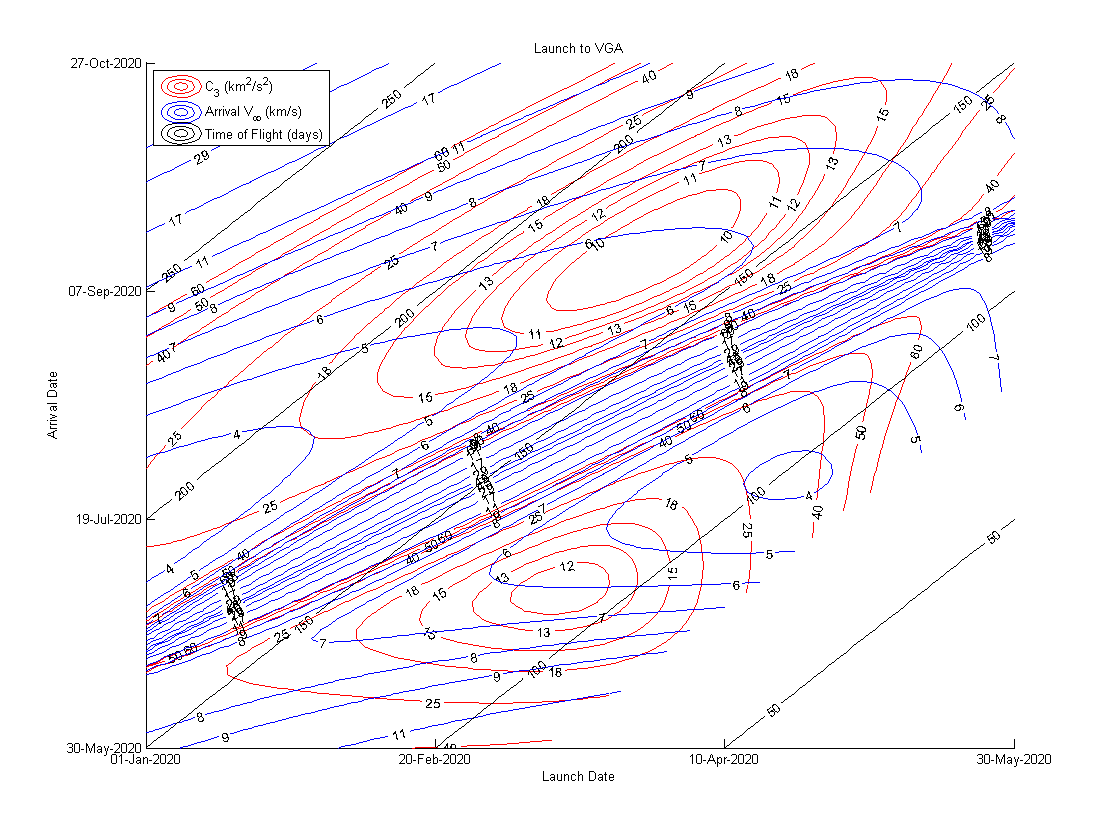
\includegraphics[width = 18cm]{../PCP/VEEJ/1_Launch_VGA.png}
		\caption{Launch to VGA. }
		\label{fig:PCP_Launch_VGA}
	\end{figure}	

	\begin{figure}[H]
		\centering
			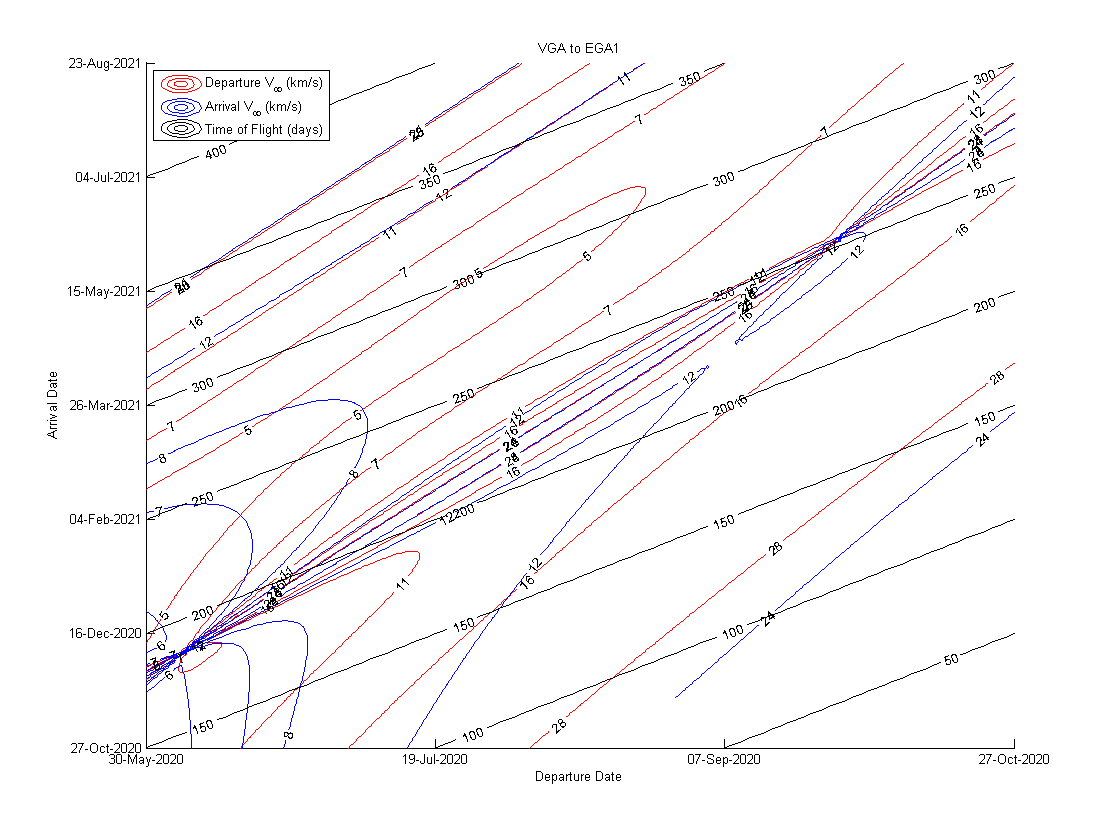
\includegraphics[width = 18cm]{../PCP/VEEJ/2_VGA_EGA1.png}
		\caption{VGA to EGA1. }
		\label{fig:PCP_VGA_EGA1}
	\end{figure}	

	\begin{figure}[H]
		\centering
			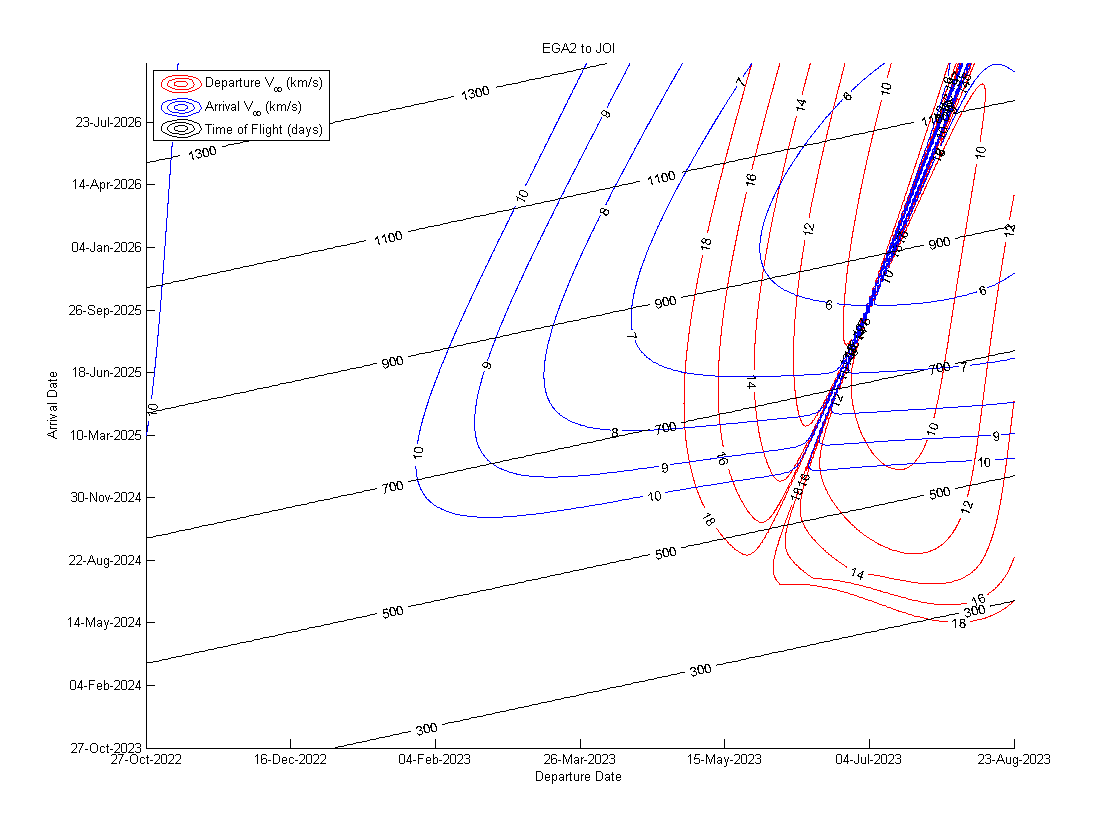
\includegraphics[width = 18cm]{../PCP/VEEJ/3_EGA2_JOI.png}
		\caption{EGA2 to JOI. }
		\label{fig:PCP_EGA2_JOI}
	\end{figure}	

	Porkchop plots serve as great visual guides to determine low-cost trajectories. However, chaining together multiple gravity assists leads to many potential solutions whose benefits become difficult to compare using several porkchop plots. An algorithm was developed to trim the search space of the possible trajectories, as well as to determine the merits of each trajectory. The algorithm took a predetermined set of windows and determined the lambert solution between the launch, gravity assists, and orbit insertion. Next, launch C3 and final $V_\infty$ were applied to the initial and final windows to rid the search space of known unusable trajectories. The ${\Delta}V$ difference between planetary encounters on a given date were subsequently calculated; any ${\Delta}V$ difference outside of a tuned tolerance were thrown out. The result was a set of dates
	
	\vspace{5 mm}

Dates were chosen to minimize the V$_\infty$ errors in the calculated gravity assist. Table \ref{TrajParams} shows the chosen dates and the relevant targeting parameters.
% Please add the following required packages to your document preamble:
% \usepackage[table,xcdraw]{xcolor}
% If you use beamer only pass "xcolor=table" option, i.e. \documentclass[xcolor=table]{beamer}
\begin{table}[H]
\centering
\caption{Trajectory parameters}
\label{TrajParams}
\begin{tabular}{|c|c|c|l|}
\hline
\rowcolor[HTML]{C0C0C0} 
\textbf{Event}                                                           & \textbf{Calendar Date}                                                & \textbf{Julian Date} & \multicolumn{1}{c|}{\cellcolor[HTML]{C0C0C0}\textbf{Information}}                      \\ \hline
Launch                                                                   & \begin{tabular}[c]{@{}c@{}}25 February 2020 \\ 12:52:48\end{tabular}  &          2458906            & \begin{tabular}[c]{@{}l@{}}C$_3$: 16.72 $\mathrm{km^2/s^2}$\\ RLA: 108.64$^\circ$\\ DLA: 7.52$^\circ$\\ Launched from \\ Tanegashima, Japan\end{tabular} \\ \hline
\begin{tabular}[c]{@{}c@{}}Venus Gravity Assist \\ (VGA)\end{tabular}    & \begin{tabular}[c]{@{}c@{}}15 September 2020 \\ 12:00:00\end{tabular} &                     2459108 & \begin{tabular}[c]{@{}l@{}}r$_\mathrm{p}$: 23224 km\\ B$_\mathrm{T}$: 29790\\ B$_\mathrm{R}$: 4735.7\\ Turning Angle: 29.63$^\circ$ \\ V$_\infty$: 6.39 km/s\\$\Delta$V$_\infty$: 2.7298e-4 km/s\end{tabular}                           \\ \hline
\begin{tabular}[c]{@{}c@{}}Resonant Orbit\end{tabular} &  -- & -- & \begin{tabular}[c]{@{}l@{}}Resonance: 2:1 \\$\varphi$: 130.06$^\circ$ \\ V$_\infty$: 9.45 km/s\\$\Delta$V$_\infty$: 2.7298e-4 km/s\end{tabular}                           \\ \hline
\begin{tabular}[c]{@{}c@{}}Earth Gravity Assist 1 \\ (EGA1)\end{tabular} & \begin{tabular}[c]{@{}c@{}}12 July 2021 \\ 12:00:00\end{tabular}      &           2459408           & \begin{tabular}[c]{@{}l@{}}r$_\mathrm{p}$: 6745.2 km\\ B$_\mathrm{T}$: -7069.2 km\\ B$_\mathrm{R}$: -7474.7 km\\ Turning Angle: 47.00$^\circ$ \end{tabular}                           \\ \hline
\begin{tabular}[c]{@{}c@{}}Earth Gravity Assist 2 \\ (EGA2)\end{tabular} & \begin{tabular}[c]{@{}c@{}}12 July 2023 \\ 12:00:00\end{tabular}      &         2460138             & \begin{tabular}[c]{@{}l@{}}r$_\mathrm{p}$: 7079.5 km\\ B$_\mathrm{T}$:-10549 km\\ B$_\mathrm{R}$: 1472.1 km\\ Turning Angle: 45.56$^\circ$ \end{tabular}                           \\ \hline
\begin{tabular}[c]{@{}c@{}}Jupiter Orbit Insertion \\ (JOI)\end{tabular} & \begin{tabular}[c]{@{}c@{}}14 February 2026 \\ 12:00:00\end{tabular}  &                     2461086 & \begin{tabular}[c]{@{}l@{}}V$_\infty$: 5.5868 km/s\\ $\Delta$V:\\ Inclination:\\ r$_\mathrm{p}$:\end{tabular}             \\ \hline
\end{tabular}
\end{table}

As Table \ref{TrajParams} shows, the $\Delta$V$_\infty$ is quite low for each gravity assist. The resonant orbit gravity assist's $\Delta$V$_\infty$ is the error between the initial approach and final departure; the V$_\infty$ magnitude between these times is assumed to be within this error. Because the errors were non-zero, trajectory correction maneuvers (TCM) will have to be performed to allow the spacecraft to reach the calculated B-plane targets. The flyby altitude for each planet is greater than 300 km. Not only does this prevent planetary impact, it reduces drag that a TCM would have to correct. With Earth encounters, conjunction analysis should be performed to ensure there is no risk to hitting another spacecraft. In addition, one must ensure that the Moon does not interfere with or stand in the way of the trajectory. TCMs will have to account for lunar perturbations.
	
	\vspace{5 mm}

The resonant orbit periapses are shown in Figure \ref{fig:reso} below.
	\begin{figure}[H]
		\centering
			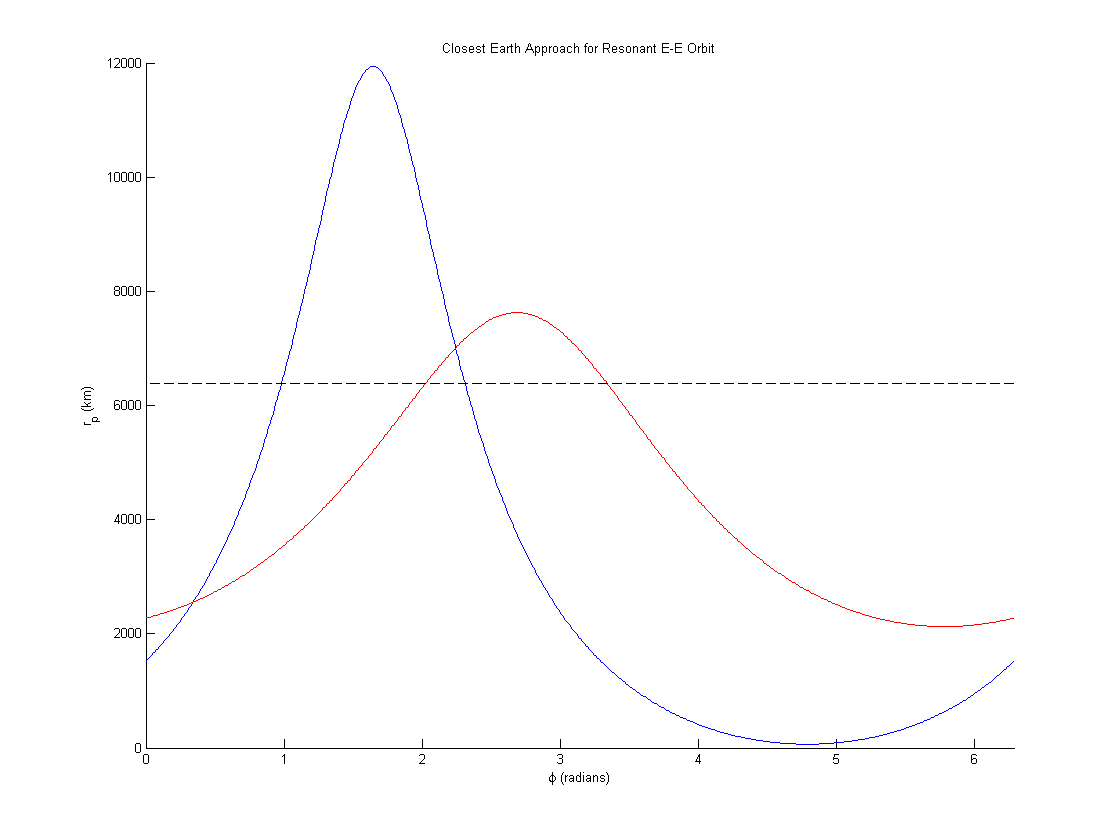
\includegraphics[width = 18cm]{../PCP/VEEJ/PhiVsRp.png}
		\caption{Resonant orbit periapses. }
		\label{fig:reso}
	\end{figure}	

The range of $\varphi$ that prevents planetary impact for both gravity assists is small. The value of $\varphi$ was chosen approximately where the periapses are the same (and greater than the radius of Earth) to ensure minimum drag effects on both flybys. 
	
	\vspace{5 mm}

A Hohmann transfer from Earth to Jupiter was constructed using semimajor axes of the planets given by Vallado\cite{Vallado} and assuming circular planetary orbits. It is shown alongside the trajectory requirements and the actual performance in Table \ref{TrajReqs} below. 
\begin{table}[H]
\centering
\caption{Trajectory requirements}
\label{TrajReqs}
\begin{tabular}{|c|c|c|c|}
\hline
\rowcolor[HTML]{C0C0C0} 
\textbf{Parameter}     & \textbf{Requirement} & \textbf{Actual}& \textbf{Hohmann} \\ \hline
Time of flight (years) & \textless10          & 6       & 2.7        \\ \hline
C3 ($\mathrm{km^2/s^2}$)              & \textless18          & 16.72     & 77.31      \\ \hline
Arrival V$_\infty$ (km/s)       & \textless6           & 5.59       & 5.64     \\ \hline
Total $\Delta$V$_\infty$ (km/s)         & \textless0.3           & 2.65e-4    & N/A     \\ \hline
\end{tabular}
\end{table}
The Hohmann transfer to Jupiter looked attractive due to the shorter time of flight, but the C$_3$ is prohibitively large. In fact, it's off the chart given by Vallado\cite{Vallado}. The proposed trajectory is most easily compared to the Galileo mission. Galileo was flown to study Jupiter and its moons; one could surmise that the mass of the spacecraft would be comparable. Like the proposed trajectory, Galileo took advantage of a VEEGA. Galileo's time of flight was just over six years. It also had a maximum C$_3$ of 17 $\mathrm{km^2/s^2}$\cite{Damario}. With a V$_\infty$ error orders of magnitude less than the maximum allowable, this trajectory was determined to be feasible.

	\section{STK Simulation}

	\section{Earth Access}

	\section{Europa Injection}

	\section{System Model}

	The equations of motion were linearized about the state $\alpha = \dot{\alpha} = \delta = \dot{\delta} =0$. Such a state was chosen because it is in equilibrium, due to the force resulting from the solar radiation pressure acting through the sailcraft's center of mass. They system is also stable about this point, as any disturbance to $\alpha$ would cause oscillation about $\alpha=0$ for a locked gimbal. The linearized equations are shown below\cite{WieSolarSail2}:

\begin{equation} \label{eq:1}
[J_s+(m_sm_p/m)b(b+l)]\ddot{\alpha}+(m_sm_p/m)bl\ddot{\delta}=-(m_p/m)bF_t-T_g+T_{ext}
\end{equation}
\begin{equation} \label{eq:2}
[J_p+(m_sm_p/m)l(b+l)]\ddot{\alpha}+[J_p+(m_sm_p/m)l^2]\ddot{\delta}=-(m_p/m)lF_t+(m_p/m)lF_n\delta+T_g
\end{equation}
	
	\vspace{5 mm}



	\section{Conclusion}

	The non-optimal controller was able to meet the design criteria without observer errors. However, it proved to not be as robust to such errors as the LQR controller. This is due to the control effort used in both controllers. The LQR design assigned a cost to control effort, so less was used. On the other hand, the non-optimal controller, which was tuned with SISO methods, was otherwise sufficient in meeting control objectives. Perhaps with sensor filtering, observer error could be reduced such that the control effort would also be reduced. 

	\vspace{5 mm}

	The Luenberger observer was able to reconstruct the entire state from only knowing the sun angle. The poles also drove initial (realistic) initial observer error to zero without forcing the actuator to violate its constraints.

	\vspace{5 mm}

	The state feedback mitigated control of the disturbance. Without the integral term, the steady-state error would be untenable for a sailcraft to get the expected thrust.  The feedback on the rest of the state ensured a quick rise that did not exceed the defined overshoot limit.

	\vspace{5 mm}

	The control methods presented were able to meet the design criteria for single-axis control of the specified solar-sail spacecraft. Further research should be done for both 2-axis gimballing and combining a gimbal with sail vanes at the edges of the sail, as well as craft with more massive busses and perhaps a gimballed payload on the other side of the sail. With such research, design flexibility will allow viable missions with reduced time or resource cost.


\bibliographystyle{aiaa}   % Number the references.
\bibliography{ASEN6008ProjectBib}   % Use references.bib to resolve the labels.

%    \section{Appendix B}
%This appendix contains all Matlab code used by the authors to analyize their data.
%    
%    \lstset{language=Matlab,%
%    	%basicstyle=\color{red},
%    	breaklines=true,%
%    	morekeywords={matlab2tikz},
%    	keywordstyle=\color{blue},%
%    	morekeywords=[2]{1}, keywordstyle=[2]{\color{black}},
%    	identifierstyle=\color{black},%
%    	stringstyle=\color{mylilas},
%    	commentstyle=\color{mygreen},%
%    	showstringspaces=false,%without this there will be a symbol in the places where there is a space
%    	numbers=left,%
%    	numberstyle={\tiny \color{black}},% size of the numbers
%    	numbersep=9pt, % this defines how far the numbers are from the text
%    	emph=[1]{for,end,break},emphstyle=[1]\color{red}, %some words to emphasise
%    	%emph=[2]{word1,word2}, emphstyle=[2]{style},   
%    }
    
%    \lstinputlisting{ASEN5090_ecef2azelrange.m}
%    \vspace{5mm}
%    
%    \lstinputlisting{ASEN5090_GPSvis.m}
%    \vspace{5mm}
%\lstinputlisting{HW5_rel_err.m}
%\vspace{5mm}
%\lstinputlisting{import_gps_data.m}
%\vspace{5mm}
%\lstinputlisting{datenum8601.m}
%\vspace{5mm}
%\lstinputlisting{lab_err_plots.m}
%\vspace{5mm}
	
\end{document}

% - Release $Name:  $ -
